



\section{Software Implementation}
The following subsections detail the implementation of the final software solution that has been written to meet the objectives posed previously of this dissertation.

\subsection{Languages and platforms}
The final system has been written entirely using the C\# programming language (version 5.0) with Visual Studio 2015 as the development environment on a Windows 10 system. C\# is an application development language built on the .NET framework. Although any number of programming languages could have been used to implement the solution C\# offered a good compromise for developing a system with both structural rigidity through static typing and object orientation in addition to functionality to allow for rapid prototyping. C\# does this well through use of LINQ, a part of the standard library that provides a large number of higher order functions which allow for operations to be performed over any data structure that implements the built in IEnumerable interface. Given that much of the code within the project performs the same operation on collections of nodes and elements stored in lists, arrays and dictionaries which all implement IEnumerable the ability to write much of the project using this capability dramatically reduced the number of errors encountered and increased development speed.


\subsection{Implementation Methodology}
The growing size of the software meant it was important to work systematically to continuously drive the project in the right direction and avoid the introduction of unnecessary complexity. This was achieved through regularly reviewing and refactoring the code which dramatically helped to reduced the amount of bugs introduced. \\

\noindent
For the duration of the project the spiral methodology was adhered to. This enforced multiple deliverable stages that were concluded with a supervisor meeting every one or two weeks. Adopting the spiral methodology also provided flexibility regarding the order in which tasks were able to take place outside of a spiral iteration. This was necessary when conducting a research driven project where direction of work for subsequent development iterations was largely driven by the  findings of the work in the previous ones. \\

\noindent
Tasks were chosen every week for the project, the number of tasks and their complexity was determined using a combination of factors including the time they were expected to take along with their criticality within the project. In a busy week requiring lots of work for other modules the tasks with lower time costs and higher criticality were typically selected over the others.

\subsection{Stress Based Refinement}
To focus meshing in areas of high stress each iteration needed to parse the results file from the previous iterations execution of LISA. LISA result files are in csv format by default and contain the displacements and stresses associated with each node within the model once it has been solved. \\

\noindent
Once the data in the output file has been parsed the nodal values for which displacement is known for can be cross referenced against those in the current model by intersecting the lists of node data on node Ids. An evaluation function is then able to determine whether or not any element handed to it meets the criteria for refinement by simply looking at the sum of the stress at its given nodes. If an element is determined to be over the threshold to justify refinement the elements ``createChildElements()'' method is called to subdivide it further. \\


\subsection{Heuristic/Rule Based Refinement}
Each rule is represented as a function within the implementation, this closely resembles the format presented by Dolsak \cite{DolsakPaper91, DolsakPaper94, appOfILPToFEMeshDesign, ConsultRuleIntellSystemFE}. The rules resides within the ``RuleManager'' class and each take a number of the defined edges as parameters. When an instance of the RuleManager is created it parses the edges file provided by the user into a list of edges that the rules can then be executed on. Every rule then checks the properties of a particular edge against properties which have been identified through the ILP learning algorithm as being important when the model executes. In cases where the rules accept more than one edge as an argument the system attempts to apply the rule to each pair of different edges in the edge list giving a time complexity of $O(n^2)$ where n is the total number of defined edges.\\

\noindent
If a rule detects a relationship in the model the edge is assigned a criticality rating as defined by the rule, the value is then used by the meshing procedure to determine how many times it should re mesh the elements along that edge. \\ 
 
\noindent
The properties that can exist between two edges when compared are the following:
\begin{itemize}
\item Edges opposite one another - The edges run alongside one another closely, look at the distance between each of the corresponding nodes and check whether this distance is less than some threshold amount.

\item Edges posses the same form - The Edges share the same edge type as one another
%finish this

\item Edges are considered the same - Both edges must be almost the same length, opposite one another and posses the same form.
\end{itemize}

\noindent
Each edge specification has several properties which Dolsak describes within his papers including:
\begin{itemize}
\item Id number - used to identify edge uniquely within the RuleManager 
\item Edge type - How would the engineer describe the edge, does it form a circuit, it an important aspect of the models design or is it along the edge of some hole?
\item Load type - Is the edge between to areas with forces applied to them, is just one side of it or is it located elsewhere within the model.
\item Boundary type - Does the edge run along a constraint point where the model is attached to the outside world.


%\colorbox{yellow}{Still need to write about this}
\end{itemize}

\noindent
Each of the three edge type properties have a set of recognised values defined by Dolsak within his paper which have been listed in appendix C. In addition to these properties used by the refinement system for deciding where to mesh each element also contains a list of nodes referencing those within the model which describe the path the edge takes along the mesh.\\


\noindent
Since this system relied on a persistent definition of edges across multiple refinement iterations another challenge was to correctly redefine edges in terms of the newly created nodes so that after meshing had occurred the rules could be re applied to a refined edge to potentially refine it further.

\begin{figure}[H]
\centering
\begin{subfigure}{.5\textwidth}
  \centering
  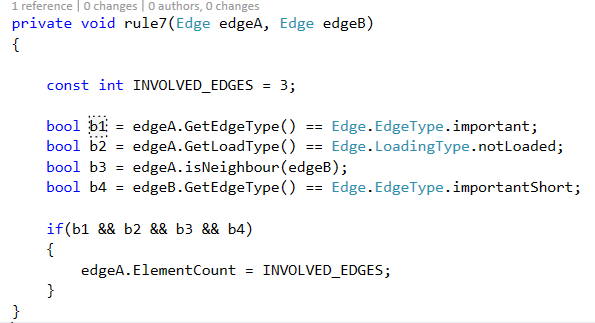
\includegraphics[width=0.9\linewidth]{../Graphics/Rule7Implementation.png}
  \caption{Code implementation of rule 7 provided by Dolsak within the RuleManger class}
  \label{fig:sub1}
\end{subfigure}%
\begin{subfigure}{.5\textwidth}
  \centering
  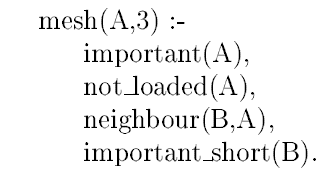
\includegraphics[width=0.7\linewidth]{../Graphics/Rule7Dolsak.png}
  \caption{Rule 7 as stated by dolsak in his papers \cite{appOfILPToFEMeshDesign}}
  \label{fig:sub2}
\end{subfigure}
\label{fig:test}
\end{figure}

\noindent
Having completed meshing of targeted areas it was also important for the heuristic refinement process to redefine the specified edges so that refinement along an edge could be performed again on a subsequent iteration taking into account the newly created nodes and their associated elements created along the original edge. The solution to this problem was yet another node traversal starting at the origin of an edge and moving through each of the node points defined along the edge while collecting newly created nodes lying between the two. \\


\noindent
Since the only information available by which to determine the new edge nodes is the node path comprising the current edge it has to be assumed that new nodes linking the each current node pair will take a direct path between the two. Since there is no graph structure stored within memory that represents all the possible traversal moves and with the number of possible paths increasing exponentially with the number of nearby nodes considered it was not practical to generate it. Consequently he only way to effectively move towards the node end point consistently was to perform a greedy search. \\ 

\noindent
The greedy search starts by computing the distance between the start and end node points for all nearby nodes, determine the nodes directly adjacent to the start and then of those nodes link the one which has the shortest distance to the end node to the path before repeating this process for that node. This approach was not the first used in an attempt to solve the problem however having completed its implementation it proved to work effectively.

%without incurring excessive runtime due to the number of potentially new nodes along an edge for each iteration only increasing quadratically. \\ 

 A more detailed pseudo code description of this process can be seen below:


\begin{algorithm}[H]
\ForAll{$E \in refinedEdges$}{
	Get the list of potentially new nodes K as the set of all nodes previously created by refining elements that run along E\; \
	
	Create a new empty list containing the new edge path used for subsequent iterations EL\;\
	
	\ForAll{$edgeNodePairs N \in E$}{
	
	Make a new sub list SL which will be the sorted path between the end of each node pairing in the current path N.FirstNode and N.SecondNode\;
	Add N.FirstNode to S\;\
	
	
	Make two lists A and B which will contain tuples holding the distance from each potentially new node to N.FirstNode in A and n2.SecondNode in B along with a reference to the potential new path node\;\

		\ForAll{$nearbyElemNode \in K$}{
			Compute euclidean distance from n1 and store with reference in A\;
			Compute euclidean distance from n2 and store with reference in B\;\
			
		
			Sort A ascending\;
			Sort B ascending\; \
			
			
			Make a list F of first n nodes from A i.e. the closest ones depending on the element type, more complex elements take higher number of nodes, in the case of quad4 take 4\;\
		
			\ForAll{$n2Node \in n2$}{
				\If{$n2Node.Ref \in F$}{
					Add	F to S\;
					Set new n1 value as F\;
					Break\;
				}
			}		
		}
		Add N.SecondNode to S to complete that section of the path\;
		Add SL to new edge path EL\;
	}
}
\caption{Greedy search of shortest node path in 3D space to form new edge path after each iteration}
\end{algorithm}


\subsection{Mesh Quality Assessment}
Dittmers rules for computing the quality of both individual elements and the entire mesh are built into their own ``MeshQualtyAssessments" and ``ElementQualityMetrics" classes, the latter of which is encapsulated within an element object, like with refinement this allows each element to assess its own quality removing the need for additional utility classes and static methods. \\

\noindent
%not sure about the last sentence here
Since each element is initialised with the nodes that comprise it, it is also possible to derive all the geometric characteristics and thus its quality metrics upon its initialisation. This allows the metrics for each element to also be calculated upon its initialisation and thus removing the risk of null values being returned when other parts of the system request this information.

\noindent
Coding the individual methods did not take too long since Dittmer provided a clear description for each metric calculation method many of the values needed to perform the calculations were also conveniently stored as properties within different parts of the model. A considerable part of calculating each metric was therefore the process of aggregating all of the necessary data from the model so that the individual values could be calculated. \\ 

\noindent
Although the element shape metrics provided an indication of how much an elements shape deviated from its ideal understanding the differences between exactly what each metric implied was challenging, specifications for the metrics did not provide information on this besides describing cases of a good value and bad value. As a consequence the metric I decided to focus my evaluation primarily on out of the ones described was the maximum corner angles which provided a clear indication of element skew. This metric was also useful in attempting to identify elements which cause problems when needing to be sorted, see 6.6.2.


%Upon evaluation of the project and concluding that effectiveness of the heuristic relied upon overlap of the %heuristically mesh area with areas of high stress


\subsection{Implementation Challenges}
Implementation of the system was not without its share of challenges, some of which required fundamentally re addressing the approach used to tackle the problem. This section outlines the main instances of such cases during the projects development where as a consequence a notable change to the implementation was made often requiring additional research.

\subsubsection{Fast Node Lookup and Update}
A key requirement for the design of the data model generated by the hierarchical re meshing process was the need to perform fast lookup of nodes already present in the mesh. Lookup is important within the meshing methods as a means of checking whether a node that is about to be created already exists within the model, in the event that no such node already exists a new one can be created however if it does then instead of creating a new node the node that already exists needs to be connected to a node in an adjacent element that is currently being refined. If nodes are not linked correctly form correct elements the physics solver is unable to assume the stress moves through one element to another despite both having nodes at the same coordinates, this results in inaccurate output or potentially an error being thrown by LISA. \\ 

\noindent
This issue arose partly as a result of the systems design, as previously mentioned subdivision for every individual element is the responsibility of that element which from a software engineering perspective is very good since it means the low level meshing process for each different type of element could be written within that elements class. This avoids the need for much heavier generalised refinement classes that would have needed to know how to perform the meshing for all elements in the model at once and for each of the different potential element types. A consequence of this was despite every Element being capable of meshing itself perfectly adjacent elements that also requiring refinement needed the ability to reconnect the new nodes along their edges to those that have been created by the adjacent element, this can be seen below in figure 9. \\ 


\begin{figure}[!h]
  \centerline{\includegraphics[width=100mm , scale=1]{../Graphics/nodeLinking.png}}
  \caption{The need for an element to check for existing adjacent nodes when subdividing itself during refinement,\\ \\
  	Orange Nodes - An original node for one or more elements \\
	Red Nodes - new nodes made by Elem A \\
	Purple Nodes - new nodes made by Elem B \\
  }
  \label{fig:h-refinementImp}
\end{figure}


\noindent
The solution to this problem was to store all the nodes in the mesh model within a C\# dictionary structure a reference to which is passed to each element within the model. The dictionary can be indexed using a Tuple of the x, y and z coordinates for the new potential element which will either return a node already at that location or indicate that no such node exists, in which case that element is then responsible for creating the node as its first instance. Dictionaries in C\# represent a generalised instance of a hash table ensuring that lookup and insert are both constant time on average.

\subsubsection{Sorting Element Nodes}
One issue faced when working with LISA was an interface requirement specified requiring nodes for each type of element to be sorted in a specific geometric order. The general rule for node ordering within LISA is to have them form a perimeter around the edge of an element in 3d space without edges crossing one another internal to the element. \\

\begin{figure}[!h]
  \centerline{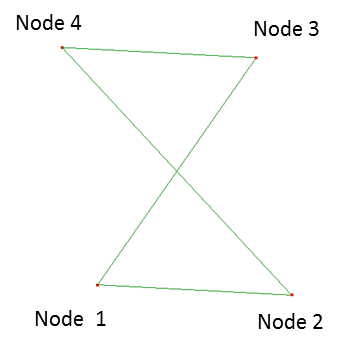
\includegraphics[width=50mm , scale=1]{../Graphics/BadlyOrderedNodes.png}}
  \caption{Element with 3d skew resulting in edges between diagonals being shortest by a small amount.
  }
  \label{fig:h-refinementImp}
\end{figure}

\noindent
When addressing this problem for simple models constructed from Quad4 elements the most straightforward approach was to simply traverse each of the nodes in the order specified by LISA and with the resulting traversal list being ordered for LISA. The resulting traversal process resembles the following: \\
	


\begin{algorithm}[H]
 make a list to contain sorted nodes called SN
 \While{$\exists node \in unstortedNodes$}{
  Get distance between current node and the next two nodes in unstortedNodes\;
  
  \eIf{sortedNodes.Count == 1}{
 	Calculate the distance between the origin node and the penultimately unsorted node A
 	Calculate the distance between the origin node and the last unsorted node B 
  	
	\eIf{lengthA > lengthB}{
		currentNode = A\;
  		Add A to SN\;
  		Remove A from unsortedNodes\;
	}
	{
		currentNode B\;
  		Add B to SN\;
  		UnstortedNodes.Remove(B)\;
	}	 
  }{
   Go through all unsorted nodes, compute distance to each, assign the node with the shortest distance as C.
    
    currentNode = C\;
  	Add c to SN
    Remove C from unsortedNodes\;
  }
 }
 \caption{A basic traversal approach for sorting Quad4 elements, code for when one node has already been sorted used to ensure that in nearly all cases the diagonal from the origin is selected as the third node in the sequence.}
\end{algorithm}

\noindent
For the most part this approach was both fast and correct for Quad4 elements although in cases where elements were particularly skewed in 3D space it was sometimes possible for an internal diagonal to be shorter than both of the edge sides as seen in Figure 9 below, this broke the traversal process which relied upon there being at least one side edge that was shorter than the diagonal. This proved to be a significant flaw in the approach and brought about the realisation that a reliable strategy for solving this problem would not be able to depend simply upon varying properties of the different elements9. \\ 

\begin{figure}[!h]
\centering
\begin{subfigure}{.5\textwidth}
  \centering
  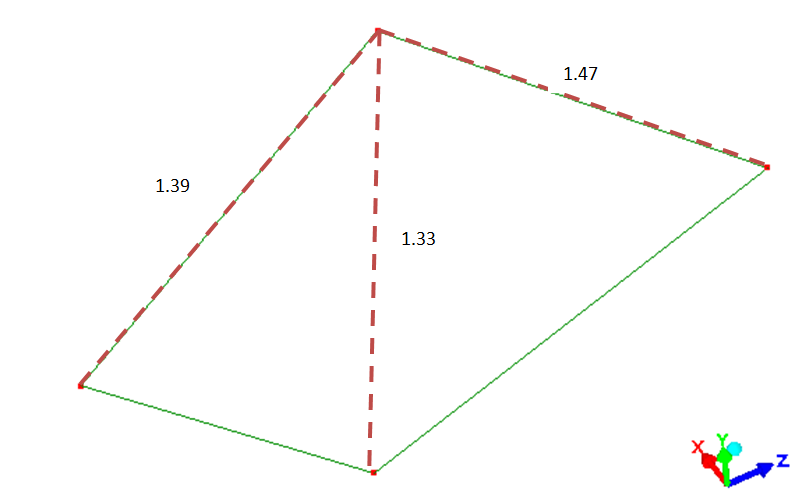
\includegraphics[width=0.9\linewidth]{../Graphics/SkewedElementIssues.png}
  \caption{Quad4 Element with diagonal shorter than both external edges}
  \label{fig:sub1}
\end{subfigure}%
\begin{subfigure}{.5\textwidth}
  \centering
  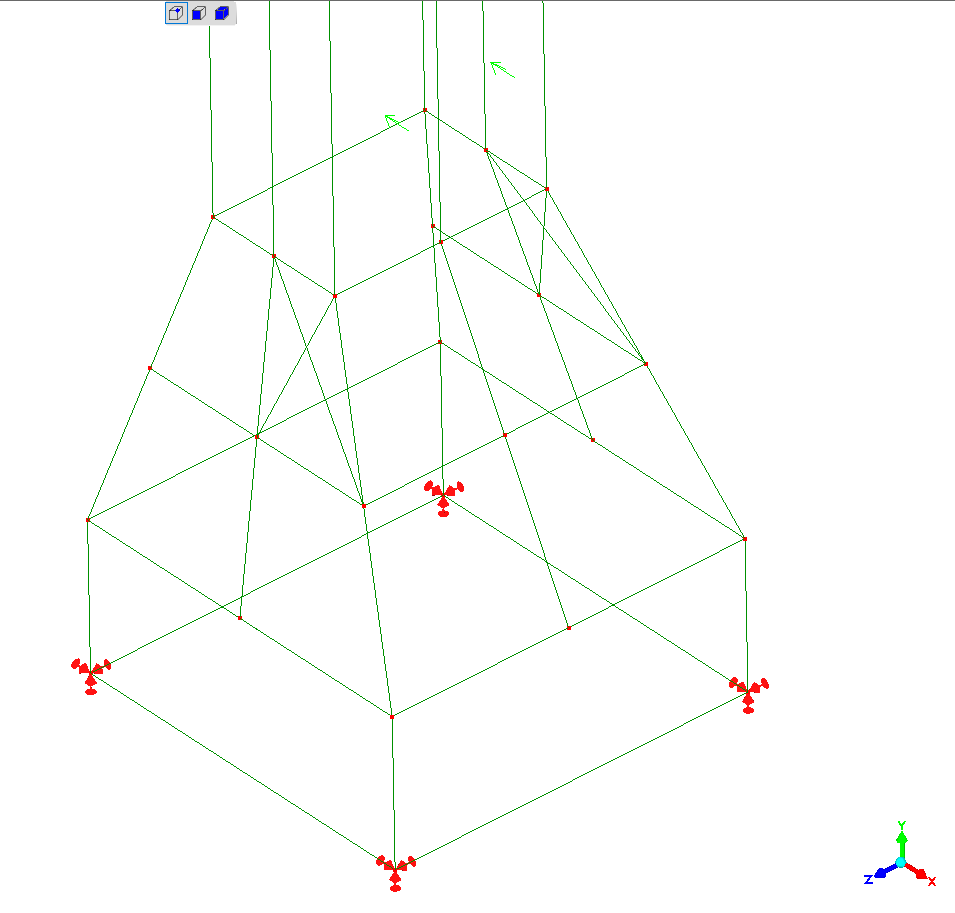
\includegraphics[width=0.7\linewidth]{../Graphics/ElementSkewOnBridge.png}
  \caption{Skew in bridge model elements resulting in rejection of the model by LISA}
  \label{fig:sub2}
\end{subfigure}
\caption{Incorrectly sorted elements arising from failure of traversal routine for skewed elements}
\label{fig:test}
\end{figure}



\noindent
Attempting to arrive at a more general solution focus was directed towards sorting the more complex Hex8 element type as this represented a more complete instance of the problem. Analysis of this led to the realisation that the most important task in sorting nodes for an arbitrary type is to simply establish the corner nodes relative to that type. Having established corners correctly sorting then simply required adding them to a list in the order specified by LISA. \\

\noindent
The subsequent method which was used to successfully establish corners for both Quad4 and Hex8 elements was to split nodes for each element using planes running along the x, y and z axis as can be seen in Figure 9 below.

\begin{figure}[!h]
\centering
\begin{subfigure}{.5\textwidth}
  \centering
  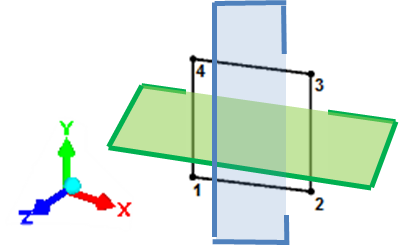
\includegraphics[width=0.9\linewidth]{../Graphics/SortingQuad4.png}
  \caption{Dividing a Quad4 along planes to establish each node as a corner point}
  \label{fig:sub1}
\end{subfigure}%
\begin{subfigure}{.5\textwidth}
  \centering
  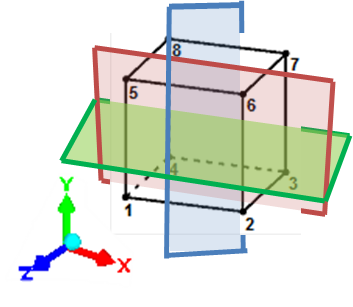
\includegraphics[width=0.7\linewidth]{../Graphics/SortingHex8.png}
  \caption{Dividing a Hex8 along planes to establish each node as a corner point}
  \label{fig:sub2}
\end{subfigure}
\caption{Splitting Element points using x, y and z planes in order to perform ordering for LISA}
\label{fig:test}
\end{figure}

\noindent
Although this approach resolved the initial problems resulting from simply trying to traverse the nodes it did not offer a strong general case solution to the problem with the code for a Hex8 element needing to be significantly different and more complex than that of a Quad4 and with the potential for the most complex FE element types such as wedge15, hex20, and pyr13 requiring implementations with even greater number of plane divisions and groupings in order to successfully identify every node. \\ 


\noindent
Having already devised two solutions it seemed likely that there would be some body of research surrounding the problem worth investigating. with research leading to a set of possible alternaives known as convex hull algorithms. As the name suggests the goal of a convex hull algorithm is to generate a convex hull, convex hulls have several definitions but the simplest of these as described by \cite{ConvexHulls} is for a set of points in some space a subset S of those points is convex if for any two points P and Q  inside S the line between the two should also be inside S. This is directly applicable in the case of quad4 elements where the LISA sort order is the convex hull of the points, in the case of more complex elements the algorithm can be applied repeatedly to different faced divided though plane splitting before sorting the nodes at the end with knowledge of node ordering within each individual face. \\ 

\begin{figure}[!h]
  \centerline{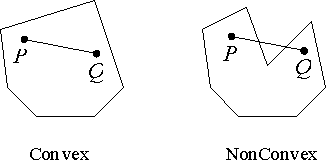
\includegraphics[width=100mm , scale=1]{../Graphics/ConvexHullGraphic.png}}
  \caption{Illustration of convex hull definition, imace source: \cite{ConvexHulls}
  }
  \label{fig:h-refinementImp}
\end{figure}

\noindent
After reviewing the different convex hull algorithms including Grapham scan \cite{GrahamScan} $O(n\ log\ n)$ and brute force scan $O(n^4)$ \cite{ConvexHulls} \cite{BruteConvex} I decided to trial the following C\# implementation of the Monotone Chain algorithm, also $O(n\ log\ n)$ \cite{CSharpConvexHull}. \\ \\ \\ \\

\noindent
The Monotone Chain algorithm algorithm was developed shortly after Graham scan and builds upon the concepts introduced in the former. Graham's scan works by initially finding the point in the data set with the lowest y coordinate which can be called P. Having found this point the other points in the set are sorted based on the angle created between them and P. Combining both these steps gives a complexity of $O(n\ log\ n)$, with  $O(n)$ to find P and $O(n\ log\ n)$ to perform a general sort of the angles. Moving through each point in the sorted array Graham scan determines whether moving to this point results in making a right or left hand turn based on the two previous points. If a right turn is made then the second do last point has caused a concave shape which has violated the requirement of the convex hull path. In this scenario is repeated the algorithm excludes the point from the convex set and resumes with the previous two points being those on the path before the rejected point. A stack structure is therefore typically used to keep track of the point ordering as is the case with the Monotone Chain implementation within the system \cite{ChainHull}. \\ 

\noindent
The Monotone Chain algorithm performs essentially the same procedure however instead of sorting using simply y values Monotone Chain sorts using both x and y values. This allows the algorithm to sort the points in two separate groups which form the top and the bottom of the hull and a reduction in the complexity of the sort comparison function. \\ \\ 

%Monotone chain
\begin{algorithm}[H]

%\begin{algorithmic}[1]
%\Procedure{Monotone Chain algorithm}{}


	Sort the points of P by x-coordinate (in case of a tie, sort by y-coordinate)\;
	%\State $\textit{U} \gets \text{Empty List}\textit{string}$
	%\State $\textit{L} \gets \text{Empty List}\textit{string}$
	Make two empty lists I and L
	Lists hold vertices of upper and lower hull\;
	
	\While{i = 1; i < n; i++}{
		\While{L contains at least two points and the sequence of last two points of L and the point P[i] does not make a counter clockwise turn}{
		Remove the last Point from L\;
		}
	}
	
	\While{i = n; i > 1; i- -}{
		\While{L contains at least two points and the sequence of last two points of L and the point P[i] does not make a counter clockwise turn}{
		
		Remove the last Point from U\;
		
		}
	}
	
Remove the last point of each list (it's the same as the first point of the other list).\;
Concatenate L and U to obtain the convex hull of P.\;
Points in the result will be listed in counter-clockwise order.\;

\caption{Monotone Chain algorithm for generating convex hull, pseudocode description credit: \cite{MonotoneChain}}\label{MonotoneChain}
\end{algorithm}

%\cite{MonotoneChain}

%algo 2


\noindent
\newline
%This method has $O(n\ log\ n)$ time complexity however due to the size of n being 4 in all cases the complexity of sorting an individual element is constant, with the overall complexity of sorting all elements in the model being $O(n)$ where n is the number of elements. \\ 

%A key drawback of both Graham scan and Monotone Chain is their limitation to 2D space. Despite the existance of algorithms for generating convex hulls in n dimensions such as \cite{} and

\noindent
The additional complexity of implementing a 3D convex hull algorithm meant it was much easier to experiment the with the approach as a potential solution to the problem using a 2D implementation by simply reducing the problem to a 2D equivalent. This was for quad4 elements by calculating the maximum delta between the max and min value on each axis and eliminating the axis with the smallest delta. These new 2D points could be given to the algorithm which when used in conjunction with the approach already taken was able to solve all instances of node ordering within the models. The only instances in which this approach failed were where highly elements would lie on a perfectly diagonal plane resulting in two axis of elimination using this method. This problem was avoid however by using the basic traversal to sort these elements. \\ 
